\chapter{Projekt Systemu Homelab}

\section{Wymagania funkcjonalne i niefunkcjonalne}

\subsection{Wymagania funkcjonalne}

\begin{enumerate}
    \item \textbf{Zarządzanie kontenerami} - możliwość konfigurowania i zarządzania kontenerami Docker w systemie, z planowaną możliwością rozszerzenia o maszyny wirtualne w przyszłości.
    \item \textbf{Panel administracyjny} - intuicyjny interfejs użytkownika stworzony przy pomocy szablonu TailAdmin\cite{TailAdmin}, umożliwiający zarządzanie zasobami systemu oraz usługami uruchamianymi w kontenerach.
    \item \textbf{Baza danych} - przechowywanie informacji o konfiguracji systemu i użytkownikach w lokalnej bazie danych SQLite.
    \item \textbf{Bezpieczny dostęp zdalny} - integracja z Tailscale umożliwiająca dostęp z dowolonego miejsca na ziemii.
    \item \textbf{Automatyzacja wdrożeń} - wsparcia dla CI/CD za pomocą GitHub Actions.
    \item \textbf{Obsługa domeny} - integracja z DuckDNS w celu dynamicznego zarządzania domeną, co umożliwia przypisanie przyjaznej nazwy do systemu HomeLab. Posiadanie własnej domeny ułatwia dostęp do usług z różnych urządzeń i lokalizacji, bez konieczności zapamiętywania adresów IP. Dodatkowo, taka domena może wskazywać zarówno na zasoby dostępne publicznie, jak i usługi działające lokalnie w prywatnej sieci domowej, co zwiększa elastyczność i komfort użytkowania.
    \item \textbf{Monitorowanie zasobów} - mechanizm zbierania infromacji o wykorzystaniu CPU, pamięci RAM oraz przestrzeni dyskowej.
    \item \textbf{Wsparcie dla rozszerzeń} - mozliwość dodawania nowych funkcji poprzez kontenery Dockera.
    \item \textbf{Łatwe wdrażanie aplikacji} - opcja uruchamiania własnych usług w kontenerach bez konieczności zaawansowanej konfiguracji.
\item \textbf{Bezpieczne uwierzytelnianie i automatyzacja} - mechanizm logowania oparty na tokenach JWT oraz zarządzanie rolami użytkowników.
\end{enumerate}

\subsection{Wymagania niefunkcjonalne}

\begin{enumerate}
    \item \textbf{Niski pobór energii} - system wdrażany jest na platformie Raspberry Pi 5, która cechuje się niskim zużyciem energii przy zachowaniu odpowiedniej wydajności. W stanie bezczynności urządzenie zużywa średnio 4-5 W \cite{RaspberryPiPowerConsumption}, natomiast podczas pełnego obciążenia zapotrzebowanie może wzrosnąć do około 12 W. Zalecane jest zasilanie 5V przy 5A (25 W), co gwarantuje stabilność działania, szczególnie podczas intensywnych operacji takich jak uruchamianie systemu czy dekodowanie wideo. Typowe zużycie prądu w trybie aktywnym wynosi około 0.8 A, a podczas rozruchu lub odtwarzania multimediów może chwilowo wzrosnąć do 1.2 A. Dzięki takim parametrom Raspberry Pi 5 stanowi idealną bazę do uruchamiania domowych systemów serwerowych przy zachowaniu niskich kosztów eksploatacji.
    \item \textbf{Wysoka dostępność} - chociaż obecna wersja systemu nie implementuje jeszcze mechanizmów redundancji, zastosowane technologie takie jak Docker oraz Tailscale VPN otwierają możliwości łatwej rozbudowy architektury o instancje uruchamiane równolegle w wielu lokalizacjach. Dzięki takiemu podejściu możliwe będzie stworzenie systemu odpornego na awarie, zapewniającego ciągłość działania nawet w przypadku niedostępności jednej z lokalizacji. Dodatkowo, rozproszenie instancji umożliwi przyszłe rozłożenie obciążenia pomiędzy węzły oraz łatwe skalowanie systemu w zależności od potrzeb użytkowników.
    \item \textbf{Łatwość w utrzymaniu} - System powinien cyklicznie sprawdzać dostępność nowej wersji aplikacji poprzez zapytania do repozytorium GitHub. W przypadku wykrycia nowego wydania, użytkownik zostanie poinformowany oraz otrzyma możliwość przeprowadzenia aktualizacji w sposób automatyczny z poziomu interfejsu użytkownika.
    \item \textbf{Skalowalność} - System wspiera również możliwość dodawania nowych usług poprzez podanie zewnętrznego repozytorium. Użytkownik może w prosty sposób wskazać adres repozytorium zawierającego plik konfiguracyjny Docker Compose, a system automatycznie zainicjuje i uruchomi kontenery na jego podstawie. Obecnie funkcjonalność ta jest ograniczona do podstawowych przypadków, jednak w planach znajduje się rozszerzenie jej o zaawansowane możliwości, takie jak integracja z istniejącymi komponentami systemu, dzielenie wspólnych baz danych pomiędzy różne kontenery oraz optymalizacja użycia zasobów, co pozwoli na minimalizację liczby uruchomionych procesów i zmniejszenie zapotrzebowania na pamięć operacyjną.
    \item \textbf{Bezpieczeństwo} - szyfrowanie komunikacji oraz kontrola dostępu do zasobów.
    \item \textbf{Modularność} - podział systemu na niezalezne komponenty działające w kontenerach Docker.
    \item \textbf{Integracja z open-source} - Wspracie dla narzędzi i trchnologii dostępnych na licencji open-source.
    \item \textbf{Minimalizacja kosztów} - niskie koszty sprzętowe i utrzymanie dzieki Raspberry Pi i rozwiązaniom chmurowym typu DuckDNS.
    \item \textbf{Wydajność} - optymalizacja aplikacji pod Raspberry Pi, aby zapenić płynne działąnie 
    \item \textbf{Łatwość wdrozenia} - uproszczona konfiguracja pozwalająca na szybkie uruchomienie systemu.
\end{enumerate}

\pagebreak

\section{Architektura systemu}
System HomeLab został zaprojektowany jako aplikacja umożliwiająca zarządzanie kontenerami Docker poprzez backend zrealizowany w języku Go, z frontendem opartym o TailAdmin oraz bazą danych SQLite. Architektura przewiduje możliwość przyszłej rozbudowy o funkcjonalność zarządzania maszynami wirtualnymi.

System HomeLab składa się z kilku kluczowych komponentów:

\begin{figure}[H]
    \centering
    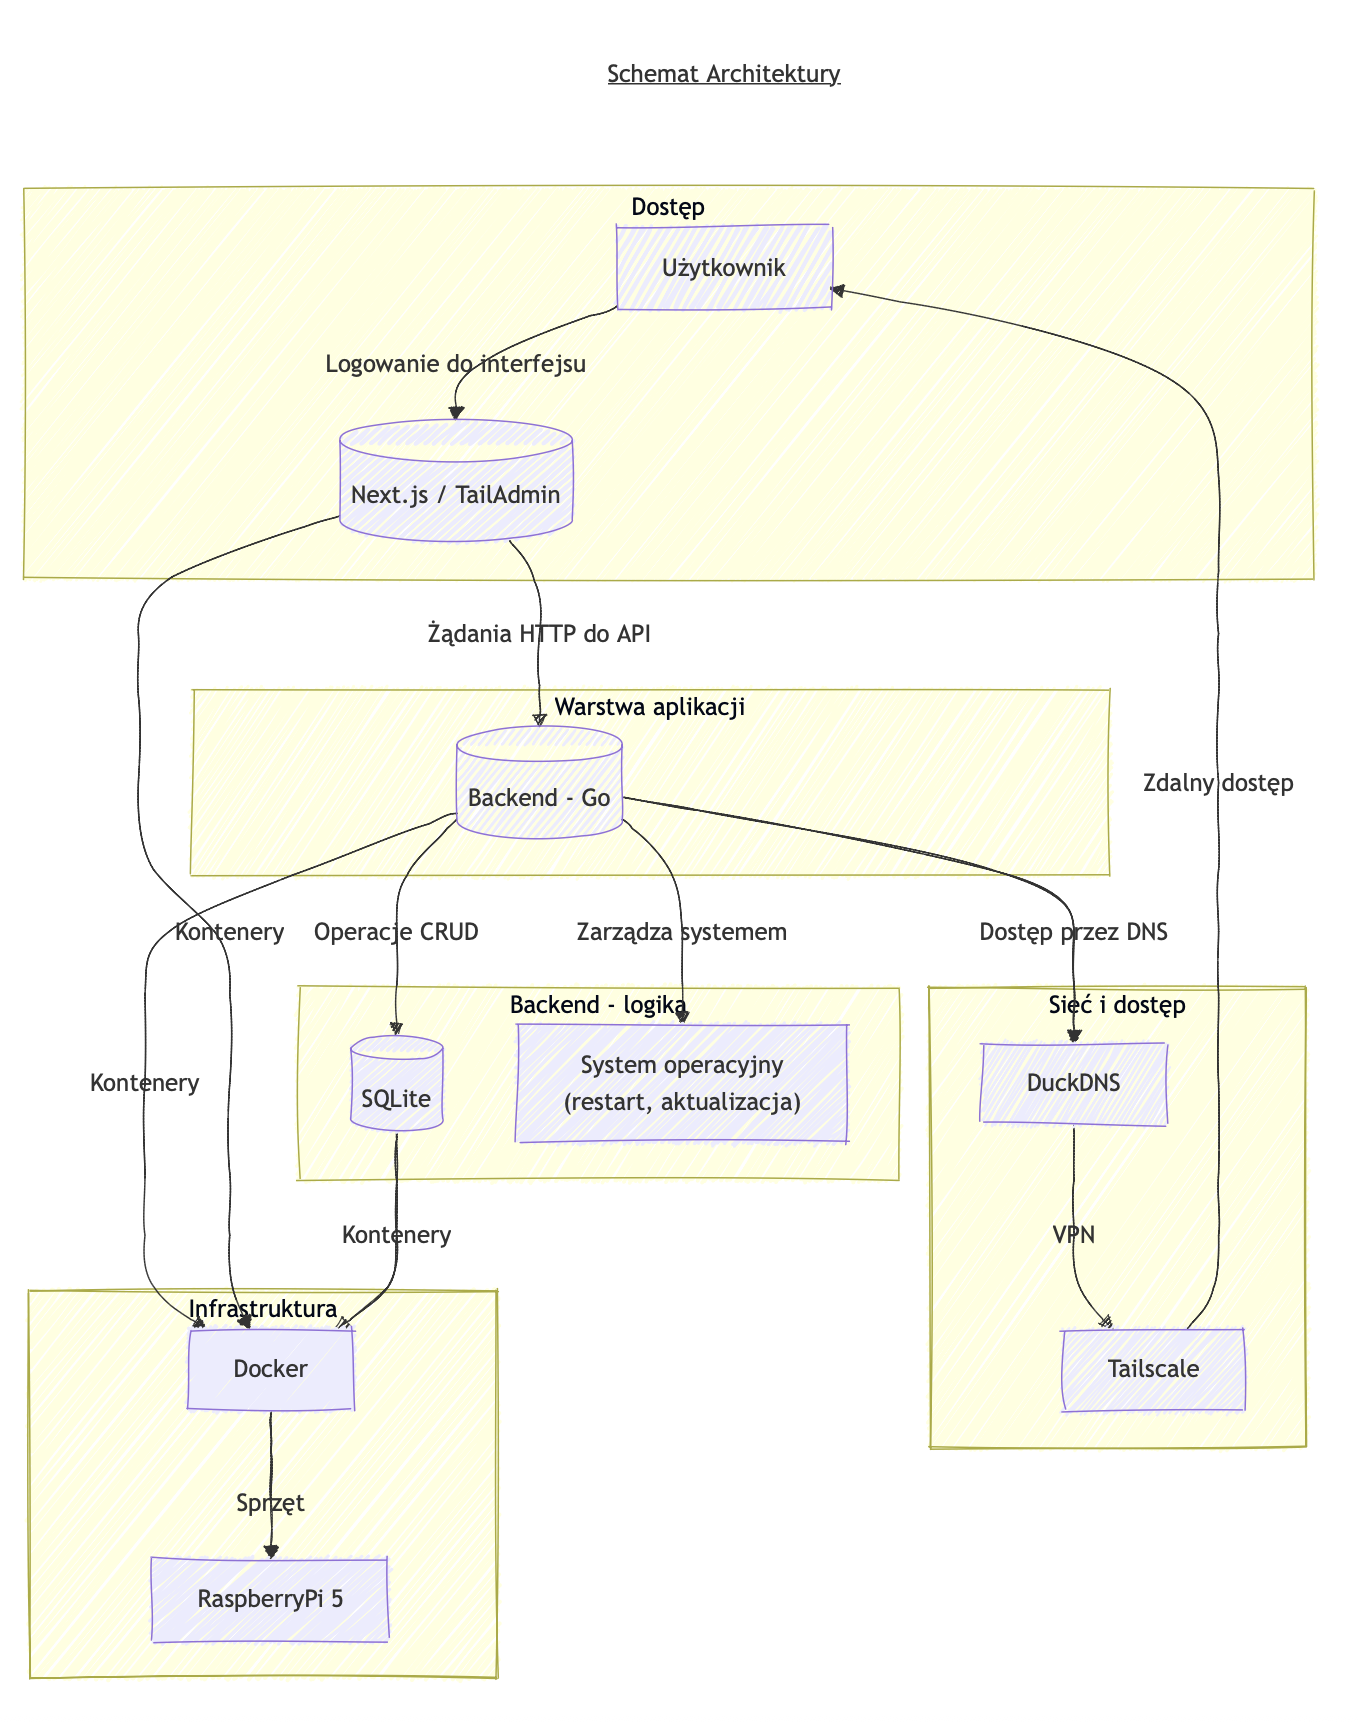
\includegraphics[width=1\textwidth]{./chapters/mermeid/schemat_architektury_updated.png}
    \caption{Schemat architektury działania i komunikacji wewnątrz stworzonego systemu.}
    \label{fig:architecture_app}
  \end{figure}

\subsection{Diagram przepływu danych}
W celu lepszego zrozumienia interakcji pomiędzy komponentami systemu, poniżej przedstawiono diagram przepływu danych ilustrujący komunikację pomiędzy frontendem, backendem, bazą danych oraz zewnętrznymi usługami:
\begin{figure}[H]
    \centering
    \includegraphics[width=0.9\textwidth]{./chapters/mermeid/schemat przepływ danych.png}
    \caption{Diagram przepływu danych w systemie HomeLab.}
    \label{fig:data_flow}
\end{figure}

\subsection{Backend (Go + SQLite)}
\begin{itemize}
    \item Backend został w całości zaimplementowany w języku Go. Odpowiada za całą logikę biznesową aplikacji oraz komunikację z systemem operacyjnym i środowiskiem kontenerowym Docker.
    \item Aplikacja backendowa zarządza stanem usług, umożliwia ich uruchamianie, zatrzymywanie oraz monitorowanie.
    \item Dane systemowe oraz informacje o użytkownikach przechowywane są lokalnie w lekkiej bazie danych SQLite, co eliminuje konieczność stosowania zewnętrznego serwera baz danych i upraszcza wdrożenie.
    \item Backend może być uruchamiany zarówno jako kontener Docker, jak i jako lokalna aplikacja zainstalowana bezpośrednio na systemie operacyjnym.
\end{itemize}

\textbf{Przykładowy fragment kodu CLI w Go odpowiedzialny za start kontenera:}
\begin{verbatim}
package main

import (
    "fmt"
    "os/exec"
)

func startContainer(containerName string) error {
    cmd := exec.Command("docker", "start", containerName)
    output, err := cmd.CombinedOutput()
    if err != nil {
        return fmt.Errorf("failed to start container: %s, %v", output, err)
    }
    fmt.Printf("Container %s started successfully\n", containerName)
    return nil
}

func main() {
    if err := startContainer("homelab_service"); err != nil {
        fmt.Println(err)
    }
}
\end{verbatim}

\subsection{Frontend (TailAdmin)}
\begin{itemize}
    \item Interfejs użytkownika oparty został o szablon TailAdmin, wykorzystujący technologię Next.js i Tailwind CSS.
    \item Frontend zapewnia nowoczesny, responsywny i intuicyjny interfejs do zarządzania usługami systemu, monitorowania zasobów i konfiguracji ustawień.
    \item Aplikacja frontendowa komunikuje się z backendem za pomocą REST API.
    \item Podobnie jak backend, może być uruchamiana jako kontener lub jako statyczna aplikacja hostowana lokalnie.
\end{itemize}

\textbf{Przykładowy fragment kodu React/JSX używanego do pobrania danych systemowych:}
\begin{verbatim}
import React, { useEffect, useState } from 'react';

function SystemStatus() {
  const [status, setStatus] = useState(null);

  useEffect(() => {
    fetch('/api/system/status')
      .then(res => res.json())
      .then(data => setStatus(data))
      .catch(err => console.error(err));
  }, []);

  if (!status) return <div>Loading...</div>;

  return (
    <div>
      <h2>Status Systemu</h2>
      <p>CPU: {status.cpuUsage}%</p>
      <p>RAM: {status.memoryUsage} MB</p>
      <p>Dysk: {status.diskSpace} GB wolne</p>
    </div>
  );
}

export default SystemStatus;
\end{verbatim}

\subsection{Warstwa sieciowa}
\begin{itemize}
    \item Połączenia z systemem realizowane są za pomocą sieci VPN opartej o Tailscale, co zapewnia bezpieczny zdalny dostęp bez konieczności stosowania przekierowań portów i stałych adresów IP.
    \item DuckDNS służy jako system dynamicznego DNS, umożliwiając dostęp do systemu za pomocą przyjaznej domeny.
\end{itemize}
\subsubsection{Topologia sieci HomeLaba}
Aby lepiej zobrazować środowisko, w którym działa system HomeLab, przedstawiono przykładową mapę sieci urządzeń i połączeń w typowej konfiguracji domowej. Schemat ilustruje powiązania między kluczowymi komponentami: serwerem głównym, NAS-em, Raspberry Pi, urządzeniami użytkownika oraz systemami zdalnego dostępu.

\begin{figure}[H]
\centering
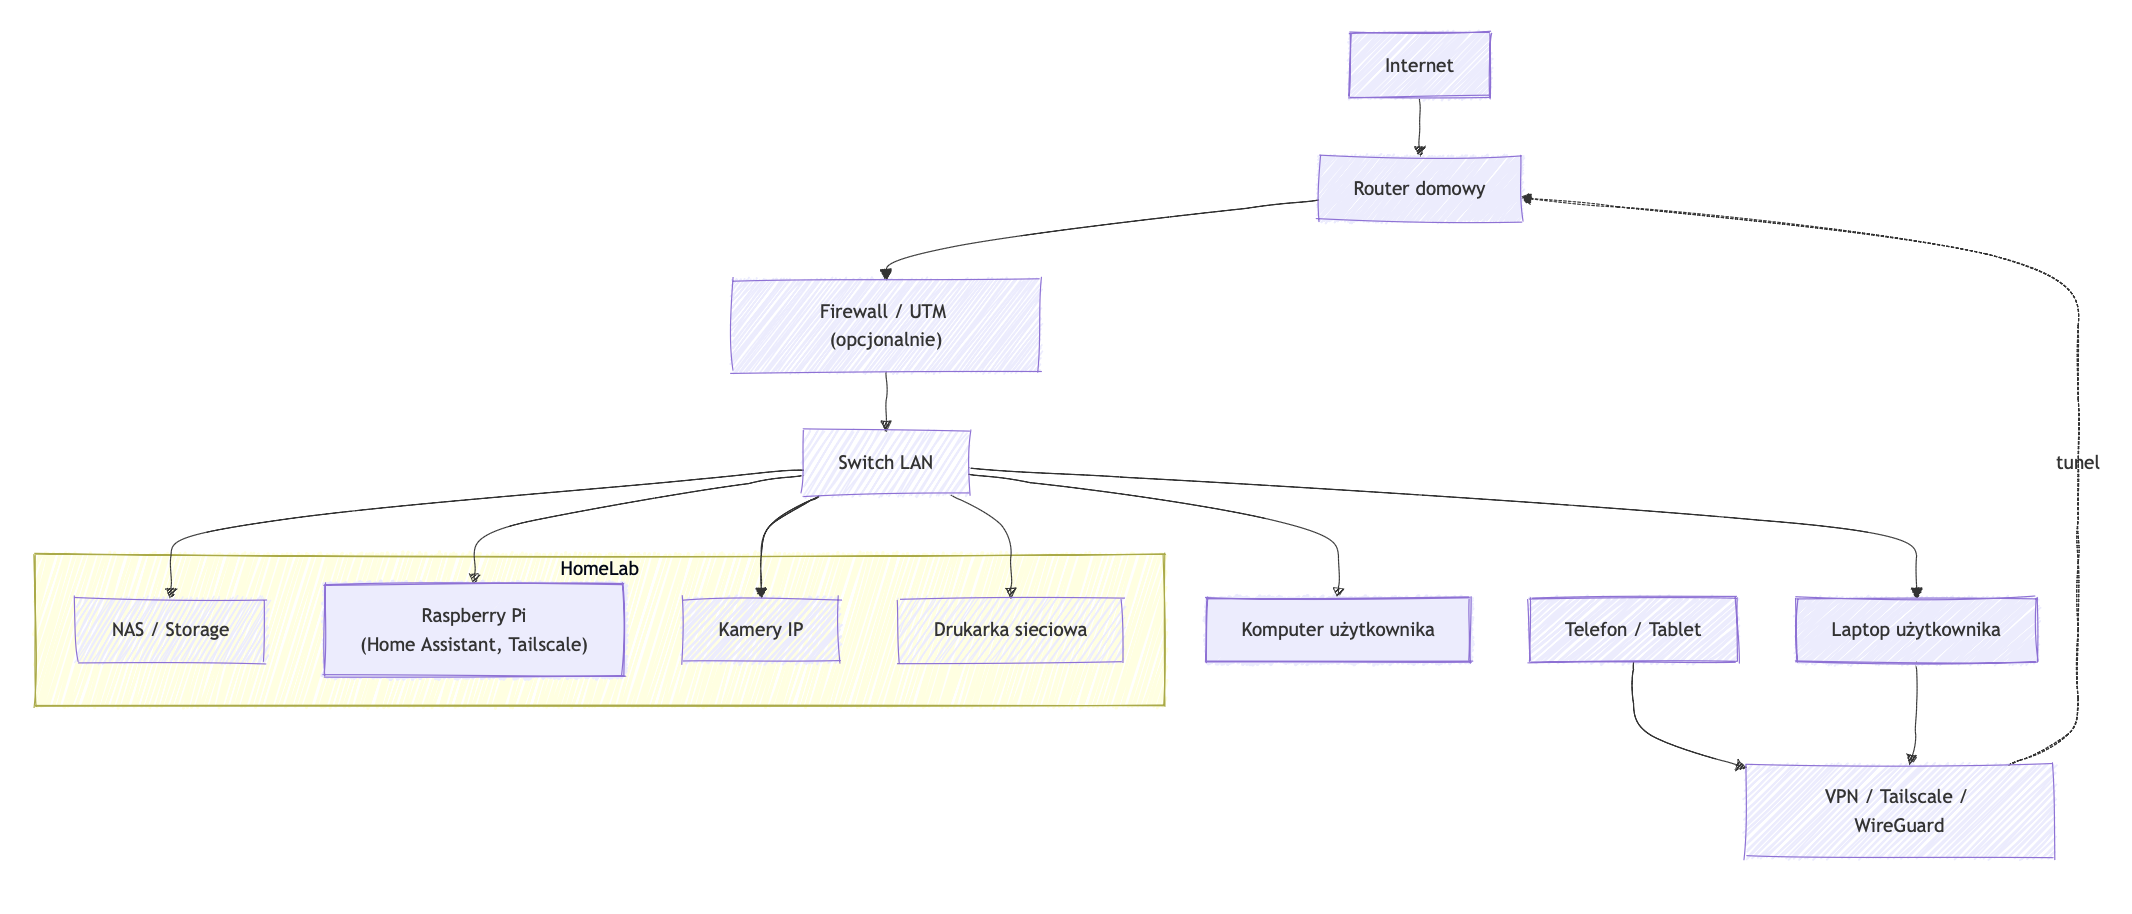
\includegraphics[width=0.95\textwidth]{./chapters/mermeid/schemat sieci homelab.png}
\caption{Mapa sieci HomeLaba z uwzględnieniem kluczowych komponentów i połączeń.}
\label{fig:network_map}
\end{figure}
\textbf{Przykładowa konfiguracja Tailscale z urządzeniem:}

\begin{verbatim}
# Instalacja Tailscale na Raspberry Pi
curl -fsSL https://tailscale.com/install.sh | sh

# Uruchomienie i logowanie do sieci Tailscale
sudo tailscale up --authkey tskey-xxxxxxxxxxxx

# Sprawdzenie statusu połączenia
tailscale status
\end{verbatim}

Konfiguracja umożliwia urządzeniu automatyczne połączenie się z siecią VPN Tailscale, co pozwala na bezpieczny dostęp zdalny do usług HomeLab bez konieczności konfiguracji przekierowań portów.

\subsection{Środowisko kontenerowe}
\begin{itemize}
    \item Docker wykorzystywany jest do zarządzania usługami uruchamianymi w ramach HomeLaba.
    \item System umożliwia instalowanie, uruchamianie i monitorowanie usług jako niezależnych kontenerów, bez potrzeby ręcznej ingerencji użytkownika.
    \item Sam system może być uruchamiany jako kontener lub lokalnie, ale niezależnie od tego zarządza innymi kontenerami poprzez lokalne API Dockera.
\end{itemize}

\subsection{Automatyzacja CI/CD}
\begin{itemize}
    \item GitHub Actions odpowiadają za automatyczne uruchamianie testów jednostkowych oraz analizę statyczną kodu (linter) po każdej zmianie w repozytorium.
    \item Po pomyślnym przejściu testów generowana jest nowa wersja aplikacji backendowej, frontendowej oraz instalatora.
    \item Nowa wersja publikowana jest jako release na GitHubie.
    \item Nie dochodzi do automatycznego wdrożenia na urządzeniu produkcyjnym - użytkownik sam decyduje o pobraniu i uruchomieniu nowej wersji.
\end{itemize}

\textbf{Przykładowy plik `.github/workflows/build.yml`:}
\begin{verbatim}
name: Build and Test

on:
  push:
    branches:
      - main
  pull_request:

jobs:
  build:
    runs-on: ubuntu-latest

    steps:
    - uses: actions/checkout@v3

    - name: Set up Go
      uses: actions/setup-go@v3
      with:
        go-version: 1.20

    - name: Build Backend
      run: go build -v ./backend/...

    - name: Run Backend Tests
      run: go test -v ./backend/...

    - name: Build Frontend
      run: |
        cd frontend
        npm install
        npm run build

    - name: Run Frontend Tests
      run: |
        cd frontend
        npm test

    - name: Create Release
      uses: softprops/action-gh-release@v1
      with:
        tag_name: ${{ github.ref }}
      env:
        GITHUB_TOKEN: ${{ secrets.GITHUB_TOKEN }}
\end{verbatim}

\subsection{Wizualizacja procesu CI/CD}
Dla pełnego zrozumienia cyklu automatyzacji wdrożenia systemu, przedstawiono uproszczony wykres przepływu operacji CI/CD:
\begin{figure}[H]
    \centering
    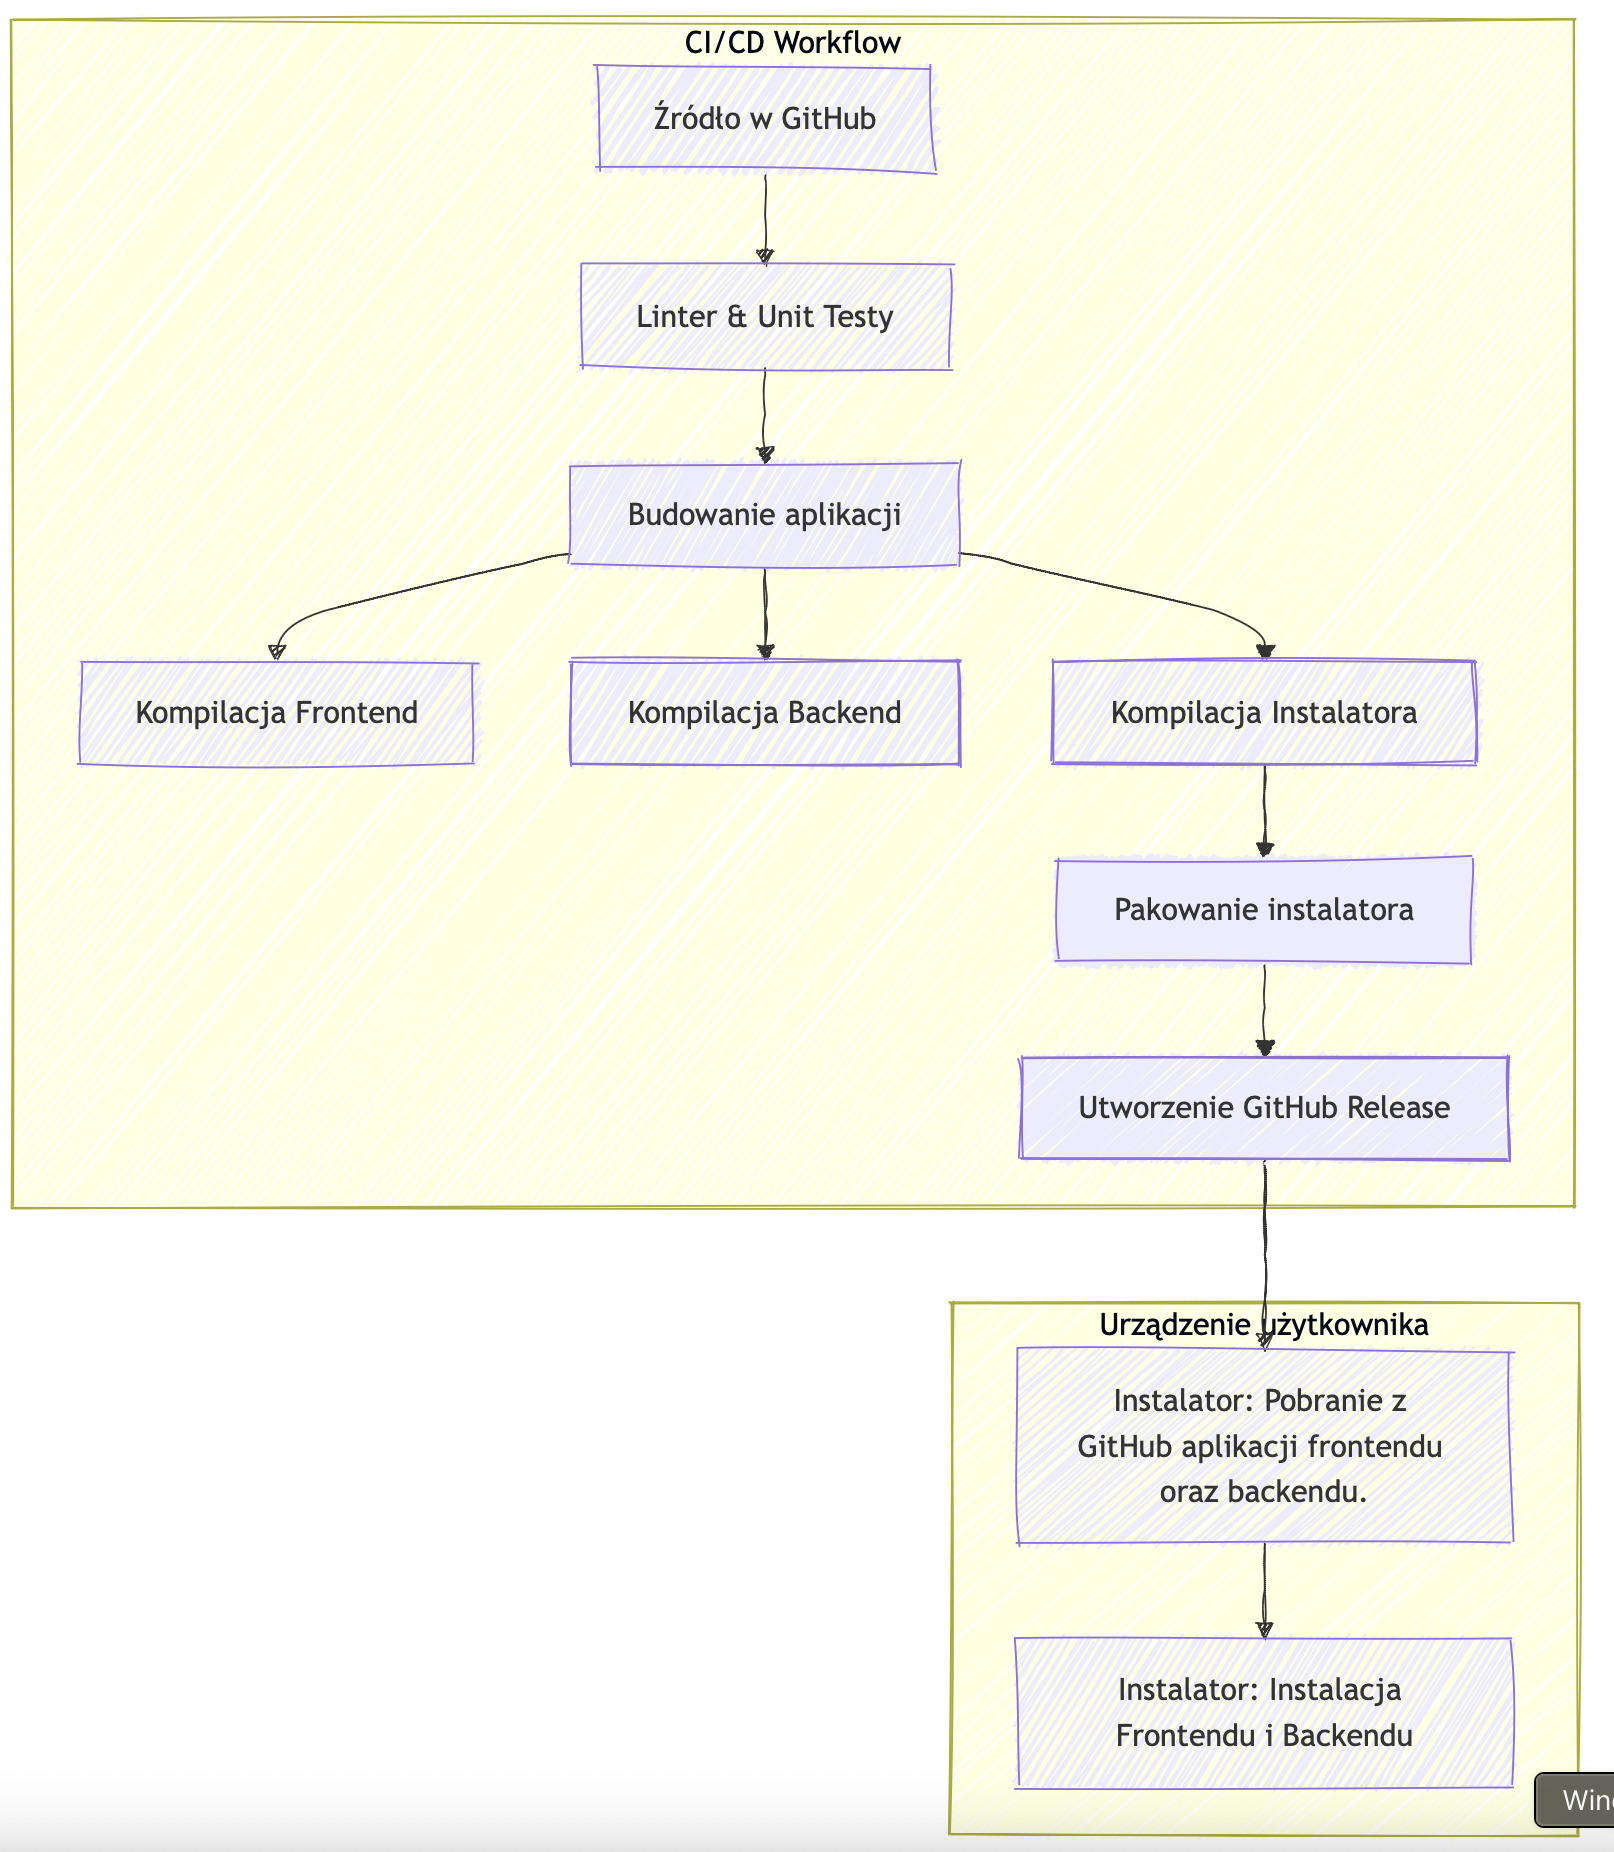
\includegraphics[width=0.95\textwidth]{./chapters/mermeid/schematcicd.png}
    \caption{Schemat procesu CI/CD od momentu zatwierdzenia zmiany aż do utworzenia wydania.}
    \label{fig:ci_cd_pipeline}
\end{figure}

\subsection{Urządzenie docelowe}

System docelowo uruchamiany jest na urządzeniu Raspberry Pi 5, które zapewnia odpowiednią wydajność przy bardzo niskim zużyciu energii. Dzięki temu możliwe jest ciągłe działanie systemu w warunkach domowych, przy minimalnych kosztach utrzymania.


\section{Technologie i narzędzia uzyte w systemie}

System HomeLab wykorzystuje następujące technologie:
\subsection{Backend}
\begin{itemize}
    \item Go - zapewnia wysoką wydajność i prostotę wdrożenia na systemach typu embedded jak Raspberry Pi.
    \item SQLite - lekka, lokalna baza danych eliminująca potrzebę zewnętrznego serwera, idealna do przechowywania konfiguracji i danych użytkowników.
\end{itemize}
\subsection{Frontend}
\begin{itemize}
    \item TailAdmin - nowoczesny szablon interfejsu użytkownika oparty na Next.js i Tailwind CSS, zapewniający responsywność i łatwość rozbudowy.
    \item REST API - umożliwia komunikację między frontendem a backendem w sposób prosty i efektywny.
\end{itemize}
\subsection{Warstwa Sieciowa}
\begin{itemize}
    \item Tailscale - VPN do bezpiecznego zapewnienia zdalnego dostępu do systemu, bez konieczności posiadania stałego adresu IP.
    \item DuckDNS - dynamiczny system zarządzania domeną umożliwiający łatwy dostęp do systemu.
\end{itemize}
\subsection{Środowisko uruchomieniowe}
\begin{itemize}
    \item Docker - uzywany do konteneryzacji aplikacji i zarządzania zależnościami, umożliwiając izolację i łatwe wdrażanie usług.
    \item Raspberry Pi 5 - host systemu zapewniający energooszczędność i niski koszt.
\end{itemize}
\subsection{Automatyzacja CI/CD}
\begin{itemize}
    \item GitHub Actions - narzędzie do automatyzacji wdrożeń i testowania kodu, umożliwiające szybkie i powtarzalne procesy buildów i testów.
    \item Pipeline CI/CD - automatyczne testowanie, budowanie i wdrażanie aplikacji, zwiększające jakość i niezawodność systemu.
\end{itemize}

Dzięki zastosowaniu powyzszych technologii system Homelab będzie nowoczesnym, skalowalnym i energooszczędnym rozwiązaniem dla uzytkowników domowych.

\section{Podsumowanie rozdziału}
W tym rozdziale szczegółowo opisano architekturę systemu HomeLab, komponenty techniczne oraz dobór technologii. Przedstawiono również sposób automatyzacji procesu wdrożenia. Na bazie tych informacji możliwa jest dalsza analiza procesu implementacji, omówiona w kolejnym rozdziale.